\documentclass[twoside]{book}

% Packages required by doxygen
\usepackage{fixltx2e}
\usepackage{calc}
\usepackage{doxygen}
\usepackage[export]{adjustbox} % also loads graphicx
\usepackage{graphicx}
\usepackage[utf8]{inputenc}
\usepackage{makeidx}
\usepackage{multicol}
\usepackage{multirow}
\PassOptionsToPackage{warn}{textcomp}
\usepackage{textcomp}
\usepackage[nointegrals]{wasysym}
\usepackage[table]{xcolor}

% Font selection
\usepackage[T1]{fontenc}
\usepackage[scaled=.90]{helvet}
\usepackage{courier}
\usepackage{amssymb}
\usepackage{sectsty}
\renewcommand{\familydefault}{\sfdefault}
\allsectionsfont{%
  \fontseries{bc}\selectfont%
  \color{darkgray}%
}
\renewcommand{\DoxyLabelFont}{%
  \fontseries{bc}\selectfont%
  \color{darkgray}%
}
\newcommand{\+}{\discretionary{\mbox{\scriptsize$\hookleftarrow$}}{}{}}

% Page & text layout
\usepackage{geometry}
\geometry{%
  a4paper,%
  top=2.5cm,%
  bottom=2.5cm,%
  left=2.5cm,%
  right=2.5cm%
}
\tolerance=750
\hfuzz=15pt
\hbadness=750
\setlength{\emergencystretch}{15pt}
\setlength{\parindent}{0cm}
\setlength{\parskip}{3ex plus 2ex minus 2ex}
\makeatletter
\renewcommand{\paragraph}{%
  \@startsection{paragraph}{4}{0ex}{-1.0ex}{1.0ex}{%
    \normalfont\normalsize\bfseries\SS@parafont%
  }%
}
\renewcommand{\subparagraph}{%
  \@startsection{subparagraph}{5}{0ex}{-1.0ex}{1.0ex}{%
    \normalfont\normalsize\bfseries\SS@subparafont%
  }%
}
\makeatother

% Headers & footers
\usepackage{fancyhdr}
\pagestyle{fancyplain}
\fancyhead[LE]{\fancyplain{}{\bfseries\thepage}}
\fancyhead[CE]{\fancyplain{}{}}
\fancyhead[RE]{\fancyplain{}{\bfseries\leftmark}}
\fancyhead[LO]{\fancyplain{}{\bfseries\rightmark}}
\fancyhead[CO]{\fancyplain{}{}}
\fancyhead[RO]{\fancyplain{}{\bfseries\thepage}}
\fancyfoot[LE]{\fancyplain{}{}}
\fancyfoot[CE]{\fancyplain{}{}}
\fancyfoot[RE]{\fancyplain{}{\bfseries\scriptsize Generated by Doxygen }}
\fancyfoot[LO]{\fancyplain{}{\bfseries\scriptsize Generated by Doxygen }}
\fancyfoot[CO]{\fancyplain{}{}}
\fancyfoot[RO]{\fancyplain{}{}}
\renewcommand{\footrulewidth}{0.4pt}
\renewcommand{\chaptermark}[1]{%
  \markboth{#1}{}%
}
\renewcommand{\sectionmark}[1]{%
  \markright{\thesection\ #1}%
}

% Indices & bibliography
\usepackage{natbib}
\usepackage[titles]{tocloft}
\setcounter{tocdepth}{3}
\setcounter{secnumdepth}{5}
\makeindex

% Hyperlinks (required, but should be loaded last)
\usepackage{ifpdf}
\ifpdf
  \usepackage[pdftex,pagebackref=true]{hyperref}
\else
  \usepackage[ps2pdf,pagebackref=true]{hyperref}
\fi
\hypersetup{%
  colorlinks=true,%
  linkcolor=blue,%
  citecolor=blue,%
  unicode%
}

% Custom commands
\newcommand{\clearemptydoublepage}{%
  \newpage{\pagestyle{empty}\cleardoublepage}%
}

\usepackage{caption}
\captionsetup{labelsep=space,justification=centering,font={bf},singlelinecheck=off,skip=4pt,position=top}

%===== C O N T E N T S =====

\begin{document}

% Titlepage & ToC
\hypersetup{pageanchor=false,
             bookmarksnumbered=true,
             pdfencoding=unicode
            }
\pagenumbering{roman}
\begin{titlepage}
\vspace*{7cm}
\begin{center}%
{\Large My Project }\\
\vspace*{1cm}
{\large Generated by Doxygen 1.8.11}\\
\end{center}
\end{titlepage}
\clearemptydoublepage
\tableofcontents
\clearemptydoublepage
\pagenumbering{arabic}
\hypersetup{pageanchor=true}

%--- Begin generated contents ---
\chapter{Hierarchical Index}
\section{Class Hierarchy}
This inheritance list is sorted roughly, but not completely, alphabetically\+:\begin{DoxyCompactList}
\item \contentsline{section}{Fruit}{\pageref{classFruit}}{}
\begin{DoxyCompactList}
\item \contentsline{section}{Apple}{\pageref{classApple}}{}
\item \contentsline{section}{Grape}{\pageref{classGrape}}{}
\item \contentsline{section}{Orange}{\pageref{classOrange}}{}
\end{DoxyCompactList}
\item \contentsline{section}{List}{\pageref{classList}}{}
\item \contentsline{section}{List\+:\+:Node}{\pageref{structList_1_1Node}}{}
\end{DoxyCompactList}

\chapter{Class Index}
\section{Class List}
Here are the classes, structs, unions and interfaces with brief descriptions\+:\begin{DoxyCompactList}
\item\contentsline{section}{\hyperlink{structnode}{node} }{\pageref{structnode}}{}
\item\contentsline{section}{\hyperlink{structnode1}{node1} }{\pageref{structnode1}}{}
\item\contentsline{section}{\hyperlink{structnode__info}{node\+\_\+info} }{\pageref{structnode__info}}{}
\end{DoxyCompactList}

\chapter{File Index}
\section{File List}
Here is a list of all files with brief descriptions\+:\begin{DoxyCompactList}
\item\contentsline{section}{\hyperlink{Lab1_8c}{Lab1.\+c} }{\pageref{Lab1_8c}}{}
\end{DoxyCompactList}

\chapter{Class Documentation}
\hypertarget{classBSD__RND}{}\section{B\+S\+D\+\_\+\+R\+ND Class Reference}
\label{classBSD__RND}\index{B\+S\+D\+\_\+\+R\+ND@{B\+S\+D\+\_\+\+R\+ND}}


Inheritance diagram for B\+S\+D\+\_\+\+R\+ND\+:
\nopagebreak
\begin{figure}[H]
\begin{center}
\leavevmode
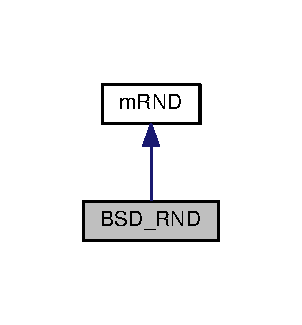
\includegraphics[width=145pt]{classBSD__RND__inherit__graph}
\end{center}
\end{figure}


Collaboration diagram for B\+S\+D\+\_\+\+R\+ND\+:
\nopagebreak
\begin{figure}[H]
\begin{center}
\leavevmode
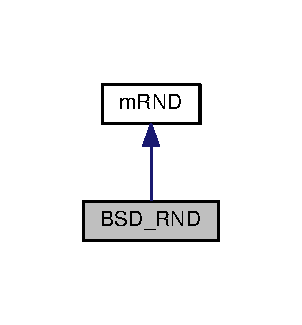
\includegraphics[width=145pt]{classBSD__RND__coll__graph}
\end{center}
\end{figure}
\subsection*{Public Member Functions}
\begin{DoxyCompactItemize}
\item 
\hyperlink{classBSD__RND_a5a8837517c5787cde6b2e0d3650c873d}{B\+S\+D\+\_\+\+R\+ND} ()
\item 
int \hyperlink{classBSD__RND_ae9e9c4d2fe83f34692f512908d2630c0}{rnd} ()
\end{DoxyCompactItemize}
\subsection*{Additional Inherited Members}


\subsection{Constructor \& Destructor Documentation}
\index{B\+S\+D\+\_\+\+R\+ND@{B\+S\+D\+\_\+\+R\+ND}!B\+S\+D\+\_\+\+R\+ND@{B\+S\+D\+\_\+\+R\+ND}}
\index{B\+S\+D\+\_\+\+R\+ND@{B\+S\+D\+\_\+\+R\+ND}!B\+S\+D\+\_\+\+R\+ND@{B\+S\+D\+\_\+\+R\+ND}}
\subsubsection[{\texorpdfstring{B\+S\+D\+\_\+\+R\+N\+D()}{BSD_RND()}}]{\setlength{\rightskip}{0pt plus 5cm}B\+S\+D\+\_\+\+R\+N\+D\+::\+B\+S\+D\+\_\+\+R\+ND (
\begin{DoxyParamCaption}
{}
\end{DoxyParamCaption}
)\hspace{0.3cm}{\ttfamily [inline]}}\hypertarget{classBSD__RND_a5a8837517c5787cde6b2e0d3650c873d}{}\label{classBSD__RND_a5a8837517c5787cde6b2e0d3650c873d}

\begin{DoxyCode}
45         \{
46             \hyperlink{classmRND_a96a1801422b5e22ac46da273b9ac68cf}{\_a} = 1103515245;
47             \hyperlink{classmRND_acfb6e24a4a40bd036057d667efb5f15c}{\_c} = 12345;
48         \}
\end{DoxyCode}


\subsection{Member Function Documentation}
\index{B\+S\+D\+\_\+\+R\+ND@{B\+S\+D\+\_\+\+R\+ND}!rnd@{rnd}}
\index{rnd@{rnd}!B\+S\+D\+\_\+\+R\+ND@{B\+S\+D\+\_\+\+R\+ND}}
\subsubsection[{\texorpdfstring{rnd()}{rnd()}}]{\setlength{\rightskip}{0pt plus 5cm}int B\+S\+D\+\_\+\+R\+N\+D\+::rnd (
\begin{DoxyParamCaption}
{}
\end{DoxyParamCaption}
)\hspace{0.3cm}{\ttfamily [inline]}}\hypertarget{classBSD__RND_ae9e9c4d2fe83f34692f512908d2630c0}{}\label{classBSD__RND_ae9e9c4d2fe83f34692f512908d2630c0}

\begin{DoxyCode}
50         \{
51             \textcolor{keywordflow}{return} \hyperlink{classmRND_af757c98d18750ecf464a2748f4958ea1}{mRND::rnd}();
52         \}
\end{DoxyCode}


Here is the call graph for this function\+:
\nopagebreak
\begin{figure}[H]
\begin{center}
\leavevmode
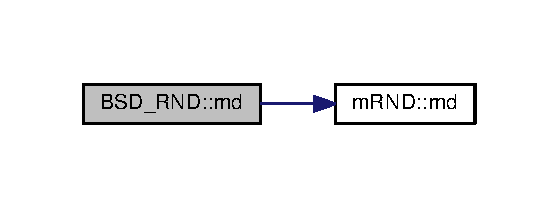
\includegraphics[width=268pt]{classBSD__RND_ae9e9c4d2fe83f34692f512908d2630c0_cgraph}
\end{center}
\end{figure}




The documentation for this class was generated from the following file\+:\begin{DoxyCompactItemize}
\item 
\hyperlink{PRNgen_8cpp}{P\+R\+Ngen.\+cpp}\end{DoxyCompactItemize}

\hypertarget{classmRND}{}\section{m\+R\+ND Class Reference}
\label{classmRND}\index{m\+R\+ND@{m\+R\+ND}}


Inheritance diagram for m\+R\+ND\+:
\nopagebreak
\begin{figure}[H]
\begin{center}
\leavevmode
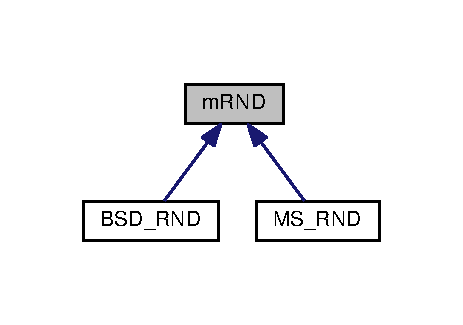
\includegraphics[width=222pt]{classmRND__inherit__graph}
\end{center}
\end{figure}
\subsection*{Public Member Functions}
\begin{DoxyCompactItemize}
\item 
void \hyperlink{classmRND_ad6c73a1c7292e22dfba539d658beab9e}{seed} (unsigned int s)
\end{DoxyCompactItemize}
\subsection*{Protected Member Functions}
\begin{DoxyCompactItemize}
\item 
\hyperlink{classmRND_ad1fb0b9caed5cb4378ae41f31f712f88}{m\+R\+ND} ()
\item 
int \hyperlink{classmRND_af757c98d18750ecf464a2748f4958ea1}{rnd} ()
\end{DoxyCompactItemize}
\subsection*{Protected Attributes}
\begin{DoxyCompactItemize}
\item 
int \hyperlink{classmRND_a96a1801422b5e22ac46da273b9ac68cf}{\+\_\+a}
\item 
int \hyperlink{classmRND_acfb6e24a4a40bd036057d667efb5f15c}{\+\_\+c}
\item 
unsigned int \hyperlink{classmRND_a77107d3df520656372e80e8934bc93bc}{\+\_\+m}
\item 
unsigned int \hyperlink{classmRND_a7c8375524993fb98192122643deac7d7}{\+\_\+seed}
\end{DoxyCompactItemize}


\subsection{Constructor \& Destructor Documentation}
\index{m\+R\+ND@{m\+R\+ND}!m\+R\+ND@{m\+R\+ND}}
\index{m\+R\+ND@{m\+R\+ND}!m\+R\+ND@{m\+R\+ND}}
\subsubsection[{\texorpdfstring{m\+R\+N\+D()}{mRND()}}]{\setlength{\rightskip}{0pt plus 5cm}m\+R\+N\+D\+::m\+R\+ND (
\begin{DoxyParamCaption}
{}
\end{DoxyParamCaption}
)\hspace{0.3cm}{\ttfamily [inline]}, {\ttfamily [protected]}}\hypertarget{classmRND_ad1fb0b9caed5cb4378ae41f31f712f88}{}\label{classmRND_ad1fb0b9caed5cb4378ae41f31f712f88}

\begin{DoxyCode}
14                :
15             \hyperlink{classmRND_a7c8375524993fb98192122643deac7d7}{\_seed}(0), \hyperlink{classmRND_a96a1801422b5e22ac46da273b9ac68cf}{\_a}(0), \hyperlink{classmRND_acfb6e24a4a40bd036057d667efb5f15c}{\_c}(0), \hyperlink{classmRND_a77107d3df520656372e80e8934bc93bc}{\_m}(2147483648)
16         \{
17         \}
\end{DoxyCode}


\subsection{Member Function Documentation}
\index{m\+R\+ND@{m\+R\+ND}!rnd@{rnd}}
\index{rnd@{rnd}!m\+R\+ND@{m\+R\+ND}}
\subsubsection[{\texorpdfstring{rnd()}{rnd()}}]{\setlength{\rightskip}{0pt plus 5cm}int m\+R\+N\+D\+::rnd (
\begin{DoxyParamCaption}
{}
\end{DoxyParamCaption}
)\hspace{0.3cm}{\ttfamily [inline]}, {\ttfamily [protected]}}\hypertarget{classmRND_af757c98d18750ecf464a2748f4958ea1}{}\label{classmRND_af757c98d18750ecf464a2748f4958ea1}

\begin{DoxyCode}
19         \{
20             \textcolor{keywordflow}{return} (\hyperlink{classmRND_a7c8375524993fb98192122643deac7d7}{\_seed} = (\hyperlink{classmRND_a96a1801422b5e22ac46da273b9ac68cf}{\_a} * \hyperlink{classmRND_a7c8375524993fb98192122643deac7d7}{\_seed} + \hyperlink{classmRND_acfb6e24a4a40bd036057d667efb5f15c}{\_c}) % \hyperlink{classmRND_a77107d3df520656372e80e8934bc93bc}{\_m});
21         \}
\end{DoxyCode}
\index{m\+R\+ND@{m\+R\+ND}!seed@{seed}}
\index{seed@{seed}!m\+R\+ND@{m\+R\+ND}}
\subsubsection[{\texorpdfstring{seed(unsigned int s)}{seed(unsigned int s)}}]{\setlength{\rightskip}{0pt plus 5cm}void m\+R\+N\+D\+::seed (
\begin{DoxyParamCaption}
\item[{unsigned int}]{s}
\end{DoxyParamCaption}
)\hspace{0.3cm}{\ttfamily [inline]}}\hypertarget{classmRND_ad6c73a1c7292e22dfba539d658beab9e}{}\label{classmRND_ad6c73a1c7292e22dfba539d658beab9e}

\begin{DoxyCode}
9         \{
10             \hyperlink{classmRND_a7c8375524993fb98192122643deac7d7}{\_seed} = s;
11         \}
\end{DoxyCode}


\subsection{Member Data Documentation}
\index{m\+R\+ND@{m\+R\+ND}!\+\_\+a@{\+\_\+a}}
\index{\+\_\+a@{\+\_\+a}!m\+R\+ND@{m\+R\+ND}}
\subsubsection[{\texorpdfstring{\+\_\+a}{_a}}]{\setlength{\rightskip}{0pt plus 5cm}int m\+R\+N\+D\+::\+\_\+a\hspace{0.3cm}{\ttfamily [protected]}}\hypertarget{classmRND_a96a1801422b5e22ac46da273b9ac68cf}{}\label{classmRND_a96a1801422b5e22ac46da273b9ac68cf}
\index{m\+R\+ND@{m\+R\+ND}!\+\_\+c@{\+\_\+c}}
\index{\+\_\+c@{\+\_\+c}!m\+R\+ND@{m\+R\+ND}}
\subsubsection[{\texorpdfstring{\+\_\+c}{_c}}]{\setlength{\rightskip}{0pt plus 5cm}int m\+R\+N\+D\+::\+\_\+c\hspace{0.3cm}{\ttfamily [protected]}}\hypertarget{classmRND_acfb6e24a4a40bd036057d667efb5f15c}{}\label{classmRND_acfb6e24a4a40bd036057d667efb5f15c}
\index{m\+R\+ND@{m\+R\+ND}!\+\_\+m@{\+\_\+m}}
\index{\+\_\+m@{\+\_\+m}!m\+R\+ND@{m\+R\+ND}}
\subsubsection[{\texorpdfstring{\+\_\+m}{_m}}]{\setlength{\rightskip}{0pt plus 5cm}unsigned int m\+R\+N\+D\+::\+\_\+m\hspace{0.3cm}{\ttfamily [protected]}}\hypertarget{classmRND_a77107d3df520656372e80e8934bc93bc}{}\label{classmRND_a77107d3df520656372e80e8934bc93bc}
\index{m\+R\+ND@{m\+R\+ND}!\+\_\+seed@{\+\_\+seed}}
\index{\+\_\+seed@{\+\_\+seed}!m\+R\+ND@{m\+R\+ND}}
\subsubsection[{\texorpdfstring{\+\_\+seed}{_seed}}]{\setlength{\rightskip}{0pt plus 5cm}unsigned int m\+R\+N\+D\+::\+\_\+seed\hspace{0.3cm}{\ttfamily [protected]}}\hypertarget{classmRND_a7c8375524993fb98192122643deac7d7}{}\label{classmRND_a7c8375524993fb98192122643deac7d7}


The documentation for this class was generated from the following file\+:\begin{DoxyCompactItemize}
\item 
\hyperlink{PRNgen_8cpp}{P\+R\+Ngen.\+cpp}\end{DoxyCompactItemize}

\hypertarget{classMS__RND}{}\section{M\+S\+\_\+\+R\+ND Class Reference}
\label{classMS__RND}\index{M\+S\+\_\+\+R\+ND@{M\+S\+\_\+\+R\+ND}}


Inheritance diagram for M\+S\+\_\+\+R\+ND\+:
\nopagebreak
\begin{figure}[H]
\begin{center}
\leavevmode
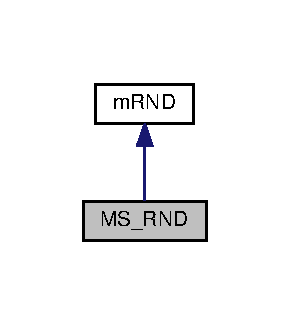
\includegraphics[width=139pt]{classMS__RND__inherit__graph}
\end{center}
\end{figure}


Collaboration diagram for M\+S\+\_\+\+R\+ND\+:
\nopagebreak
\begin{figure}[H]
\begin{center}
\leavevmode
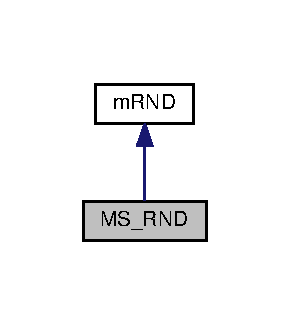
\includegraphics[width=139pt]{classMS__RND__coll__graph}
\end{center}
\end{figure}
\subsection*{Public Member Functions}
\begin{DoxyCompactItemize}
\item 
\hyperlink{classMS__RND_ad5fb4624044abfd6f9d7f2f137ff8ce0}{M\+S\+\_\+\+R\+ND} ()
\item 
int \hyperlink{classMS__RND_a5a32e10e7fac99adae8961a9ef388af3}{rnd} ()
\end{DoxyCompactItemize}
\subsection*{Additional Inherited Members}


\subsection{Constructor \& Destructor Documentation}
\index{M\+S\+\_\+\+R\+ND@{M\+S\+\_\+\+R\+ND}!M\+S\+\_\+\+R\+ND@{M\+S\+\_\+\+R\+ND}}
\index{M\+S\+\_\+\+R\+ND@{M\+S\+\_\+\+R\+ND}!M\+S\+\_\+\+R\+ND@{M\+S\+\_\+\+R\+ND}}
\subsubsection[{\texorpdfstring{M\+S\+\_\+\+R\+N\+D()}{MS_RND()}}]{\setlength{\rightskip}{0pt plus 5cm}M\+S\+\_\+\+R\+N\+D\+::\+M\+S\+\_\+\+R\+ND (
\begin{DoxyParamCaption}
{}
\end{DoxyParamCaption}
)\hspace{0.3cm}{\ttfamily [inline]}}\hypertarget{classMS__RND_ad5fb4624044abfd6f9d7f2f137ff8ce0}{}\label{classMS__RND_ad5fb4624044abfd6f9d7f2f137ff8ce0}

\begin{DoxyCode}
31         \{
32             \hyperlink{classmRND_a96a1801422b5e22ac46da273b9ac68cf}{\_a} = 214013;
33             \hyperlink{classmRND_acfb6e24a4a40bd036057d667efb5f15c}{\_c} = 2531011;
34         \}
\end{DoxyCode}


\subsection{Member Function Documentation}
\index{M\+S\+\_\+\+R\+ND@{M\+S\+\_\+\+R\+ND}!rnd@{rnd}}
\index{rnd@{rnd}!M\+S\+\_\+\+R\+ND@{M\+S\+\_\+\+R\+ND}}
\subsubsection[{\texorpdfstring{rnd()}{rnd()}}]{\setlength{\rightskip}{0pt plus 5cm}int M\+S\+\_\+\+R\+N\+D\+::rnd (
\begin{DoxyParamCaption}
{}
\end{DoxyParamCaption}
)\hspace{0.3cm}{\ttfamily [inline]}}\hypertarget{classMS__RND_a5a32e10e7fac99adae8961a9ef388af3}{}\label{classMS__RND_a5a32e10e7fac99adae8961a9ef388af3}

\begin{DoxyCode}
36         \{
37             \textcolor{keywordflow}{return} \hyperlink{classmRND_af757c98d18750ecf464a2748f4958ea1}{mRND::rnd}() >> 16;
38         \}
\end{DoxyCode}


Here is the call graph for this function\+:
\nopagebreak
\begin{figure}[H]
\begin{center}
\leavevmode
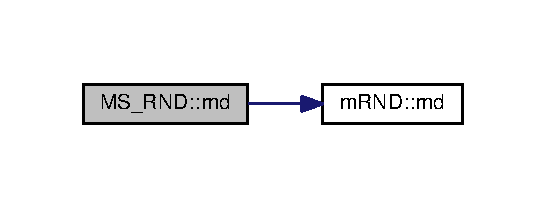
\includegraphics[width=262pt]{classMS__RND_a5a32e10e7fac99adae8961a9ef388af3_cgraph}
\end{center}
\end{figure}




The documentation for this class was generated from the following file\+:\begin{DoxyCompactItemize}
\item 
\hyperlink{PRNgen_8cpp}{P\+R\+Ngen.\+cpp}\end{DoxyCompactItemize}

\chapter{File Documentation}
\hypertarget{PRNgen_8cpp}{}\section{P\+R\+Ngen.\+cpp File Reference}
\label{PRNgen_8cpp}\index{P\+R\+Ngen.\+cpp@{P\+R\+Ngen.\+cpp}}
{\ttfamily \#include $<$iostream$>$}\\*
Include dependency graph for P\+R\+Ngen.\+cpp\+:
\nopagebreak
\begin{figure}[H]
\begin{center}
\leavevmode
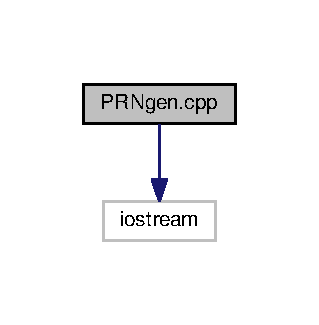
\includegraphics[width=153pt]{PRNgen_8cpp__incl}
\end{center}
\end{figure}
\subsection*{Classes}
\begin{DoxyCompactItemize}
\item 
class \hyperlink{classmRND}{m\+R\+ND}
\item 
class \hyperlink{classMS__RND}{M\+S\+\_\+\+R\+ND}
\item 
class \hyperlink{classBSD__RND}{B\+S\+D\+\_\+\+R\+ND}
\end{DoxyCompactItemize}
\subsection*{Functions}
\begin{DoxyCompactItemize}
\item 
int \hyperlink{PRNgen_8cpp_a0ddf1224851353fc92bfbff6f499fa97}{main} (int argc, char $\ast$argv\mbox{[}$\,$\mbox{]})
\end{DoxyCompactItemize}


\subsection{Function Documentation}
\index{P\+R\+Ngen.\+cpp@{P\+R\+Ngen.\+cpp}!main@{main}}
\index{main@{main}!P\+R\+Ngen.\+cpp@{P\+R\+Ngen.\+cpp}}
\subsubsection[{\texorpdfstring{main(int argc, char $\ast$argv[])}{main(int argc, char *argv[])}}]{\setlength{\rightskip}{0pt plus 5cm}int main (
\begin{DoxyParamCaption}
\item[{int}]{argc, }
\item[{char $\ast$}]{argv\mbox{[}$\,$\mbox{]}}
\end{DoxyParamCaption}
)}\hypertarget{PRNgen_8cpp_a0ddf1224851353fc92bfbff6f499fa97}{}\label{PRNgen_8cpp_a0ddf1224851353fc92bfbff6f499fa97}

\begin{DoxyCode}
56 \{
57     \hyperlink{classBSD__RND}{BSD\_RND} bsd\_rnd;
58     \hyperlink{classMS__RND}{MS\_RND} ms\_rnd;
59  
60     cout << \textcolor{stringliteral}{"MS RAND:"} << endl << \textcolor{stringliteral}{"========"} << endl;
61     \textcolor{keywordflow}{for} (\textcolor{keywordtype}{int} x = 0; x < 10; x++)
62         cout << ms\_rnd.\hyperlink{classMS__RND_a5a32e10e7fac99adae8961a9ef388af3}{rnd}() << endl;
63  
64     cout << endl << \textcolor{stringliteral}{"BSD RAND:"} << endl << \textcolor{stringliteral}{"========="} << endl;
65     \textcolor{keywordflow}{for} (\textcolor{keywordtype}{int} x = 0; x < 10; x++)
66         cout << bsd\_rnd.\hyperlink{classBSD__RND_ae9e9c4d2fe83f34692f512908d2630c0}{rnd}() << endl;
67  
68     \textcolor{keywordflow}{return} 0;
69 \}
\end{DoxyCode}


Here is the call graph for this function\+:
\nopagebreak
\begin{figure}[H]
\begin{center}
\leavevmode
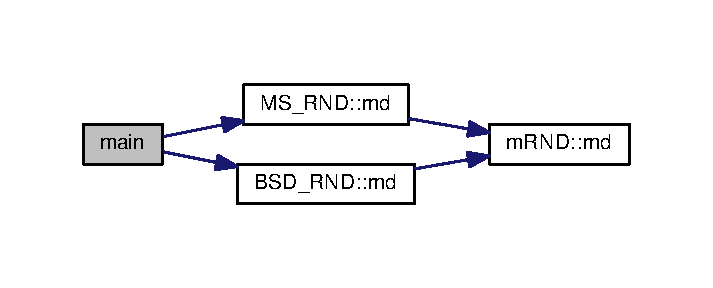
\includegraphics[width=342pt]{PRNgen_8cpp_a0ddf1224851353fc92bfbff6f499fa97_cgraph}
\end{center}
\end{figure}



%--- End generated contents ---

% Index
\backmatter
\newpage
\phantomsection
\clearemptydoublepage
\addcontentsline{toc}{chapter}{Index}
\printindex

\end{document}
